The FMM as originally presented has since been extended into a broad class of algorithms with differing implications for practical implementations. We consider the problem in its most generic form by returning to the matrix vector product (\ref{eq:n_body:sec:1_1}). Consider an $N$ body evaluation of electrostatic potentials, which motivated the development of the original FMM of Greengard and Rokhlin \cite{greengard1987fast}. We let $\{ x_i\}_{i=1}^N \in \mathbb{R}^d$ denote the set of locations of charges of strength $q_i$, where $d=2$ or $d=3$. Our task is then to evaluate potentials, $\phi_j$ for $i=1,2,...,N$. We can without loss of generality take the value of $K(x,x)=0$. Denoting our square domain containing all points with $\Omega$, we seek a matrix vector product of the form,

\begin{flalign}
    \label{eq:potential_matvec:sec_1_2}
    \mathsf{\phi} = \mathsf{K} \mathsf{q}
\end{flalign}

where $\mathsf{\phi} \in \mathbb{C}^N$, $\mathsf{q} \in \mathbb{C}^N$ and $\mathsf{K} \in \mathbb{C}^{N \times N}$. The idea is to compress the kernel interactions defined by $K(x,y)$ when $x$ and $y$ are distant. Consider the situation in figure [FIGURE OF SINGLE LEVEL SITUATION] where we choose $\mathbb{R}^2$ for simplicity. Here we seek to evaluate the potential induced by the `source particles, ${y_j}^M$, in $\Omega_s$ at the target particles, ${x_i}^L$ in $\Omega_t$. 

\begin{flalign}
    \label{eq:two_box_calc:sec_1_2}
    \phi_i = \sum_{j=1}^L K(x_i, y_j) q_j, \> \> i=1,2...M
\end{flalign}

As the sources and targets are physically distant, we can apply a low-rank approximation for the kernel as a sum of tensor products,

\begin{flalign}
    K(x,y) \approx \sum_{p=0}^{P-1}B_p(x)C_p(y), \> \> \text{when } x \in \Omega_t, y \in \Omega_s 
\end{flalign}

where $P$ is called the `expansion order', or `interaction rank'. We introduce the index sets $I_s$ and $I_t$ which list the points inside $\Omega_s$ and $\Omega_t$ respectively, and consider a generic approximation by tensor products where,

\begin{flalign}
    \hat{q}_p = \sum_{j \in I_s} C_p(x_j)q_j, \> \> p = 0,1,2,...,P-1
\end{flalign}

this is valid as $K$ is smooth in the far field. Using this, we evaluate the approximation of the potential at the targets as,

\begin{flalign}
    \label{eq:low_rank_appx:sec_1_2}
    \phi_i \approx \sum_{p=1}^{P-1} B_p(x_i)\hat{q}_p
\end{flalign}

In doing so we see that we accelerate (\ref{eq:two_box_calc:sec_1_2}) from $O(M+L)$ to $O(P(M+L))$. As long as we choose $P << M$ and $P << L$, we will recover an accelerated matrix vector product. The power of the FMM, and similar fast algorithms, is that we can recover the potential in $\Omega_t$ with high accuracy even when $P$ is small. We deliberately haven't stated how we calculate $B_p$ or $C_p$. In Greengard and Rokhlin's FMM these took the form of analytical multipole and local expansions of the kernel function \cite{greengard1987fast}. 

To demonstrate this we derive an expansion in the $\mathbb{R}^2$ case, taking $c_s$ and $c_t$ as the centres of $\Omega_s$ and $\Omega_t$ respectively,

\begin{flalign}
    \label{eq:analytical_multipole_expansion:sec_1_2}
    K(x,y) = \log(x-y) &= \log((x-c_s) - (y-c_s)) \\ \nonumber &= \log(x-c_s) + \log(1-\frac{y-c_s}{x-c_s}) \\
    \nonumber &= \log(x-c_s) - \sum_{p=1}^\infty \frac{1}{p}\frac{(y-c_s)^p}{(x-c_s)^p}
\end{flalign}

where the series converges for $|y-c_s| < |c-c_s|$. We note (\ref{eq:analytical_multipole_expansion:sec_1_2}) is exactly of the form required with $C_p(y) = -\frac{1}{p}(y-c_s)^p$ and $B_p(x) = (x-c_s)^{-p}$. We define a `multipole expansion' of the charges in $\Omega_s$ as a vector $\mathsf{\hat{q}^s} = \{ \hat{q}_p^s \}_{p=0}^{P-1}$,

\begin{flalign}
    \begin{dcases}
        \hat{q}_0^s = \sum_{j \in I_s} q_j \\ 
        \hat{q}_p^s = \sum_{j \in I_s} - \frac{1}{p}(x_j - c_s)^p q_j, \> \> p = 1,2,3...,P-1
    \end{dcases}
\end{flalign}

The multipole expansion is a representation of the charges in $\Omega_s$ and can be truncated to any required precision. We can use the multipole expansion in place of a direct calculation with the particles in $\Omega_s$. As the potential in $\Omega_t$ can be written as,

\begin{flalign}
    \phi(x) = \sum_{j \in I_s} K(x, y)q_j = \log(x-c_s)\hat{q}_0^s + \sum_{p=1}^\infty \frac{1}{(x-c_s)^p}\hat{q}_p^\sigma
\end{flalign}

Greengard and Rokhlin also define a local expansion centered on $\Omega_t$, that represents the potential due to the sources in $\Omega_s$.

\begin{flalign}
    \phi(x) = \sum_{p=1}^\infty (x-c_t)^p \hat{\phi}^t_p
\end{flalign}

with a simple computation to derive the local expansion coefficients $\{\hat{\phi}^t_p\}_{p=0}^\infty$ from $\{ \hat{q}_p^s \}_{p=0}^{P-1}$ (see app. \ref{app:a_1_fmm_algorithm}).

For our purposes it's useful to write the multipole expansion in linear algebraic terms as a linear map,

\begin{flalign}
    \mathsf{\hat{q}}^s = \mathsf{T}^{P2M}_s\mathsf{q}(I_s)    
\end{flalign}

where $\mathsf{T}_s^{P2M}$ is a $P \times N_s$ matrix, analogously for the local expansion coefficients we can write,

\begin{flalign}
    \mathsf{\hat{\phi}}^t = \mathsf{T}_{t,s}^{M2L}\mathsf{\hat{q}}^s
\end{flalign}

where $\mathsf{T}_{t,s}^{M2L}$ is a $P \times P$ matrix, and the calculation of the final potentials as,

\begin{flalign}
    \mathsf{\phi}^t = \mathsf{T}_t^{L2P}\mathsf{\hat{\phi}}^t
\end{flalign}

where $\mathsf{T}_t^{L2P}$ is a $N_t \times P$ matrix. Here we denote each \textit{translation} operator, $\mathsf{T}$, with a label read `'$X$ to $Y$' where $L$ stands for local, $M$ for multipole and $P$ for particle. Written in this form, we observe that we could use a different method to approximate the translation operators than explicit kernel expansions to recover our approach's algorithmic complexity, and this is indeed the main difference between different implementations of the FMM.

We have described how to obtain linear complexity when considering two isolated nodes, however to recover this for interactions between \textit{all particles} with we rely on a hierarchical partitioning of $\Omega$ using a data structure from computer science called a \textit{quadtree} in $\mathbb{R}^2$ or an \textit{octree} in $\textit{R}^3$. 

The defining feature of these data structures is a recursive partition of a bounding box drawn over the region of interest (see fig. \ref{fig:octree_example:sec_1_2}). This ‘root node’ is subdivided into four equal parts in $\mathbb{R}^2$ and eight equal parts in $\mathbb{R}^3$. These ‘child nodes’ turn are recursively subdivided until a user defined threshold is reached based on the maximum number of points per leaf node. These trees can be `adaptive' by allowing for non-uniform node sizes, and `balanced' to enforce a maximum size constraint between adjacent nodes \cite{sundar2008bottom}.

\gls{FMM} literature distinguishes between types of relationships  between neighbouring nodes with the concept of \textit{interaction lists}. There are four such lists for a given node $B$, called $V$, $U$, $W$ and $X$. For a leaf node $B$, the $U$ list contains $B$ itself and leaf nodes adjacent to $B$. and the $W$ list consists of the descendants of $B$'s neighbours whose parents are adjacent to $B$. For non-leaf nodes, the $V$ list is the set of children of the neighbours of the parent of $B$ which are not adjacent to $B$, and the $X$ list consists of all nodes $A$ such that $B$ is in their $W$ lists. 

\begin{figure}
    \centering
    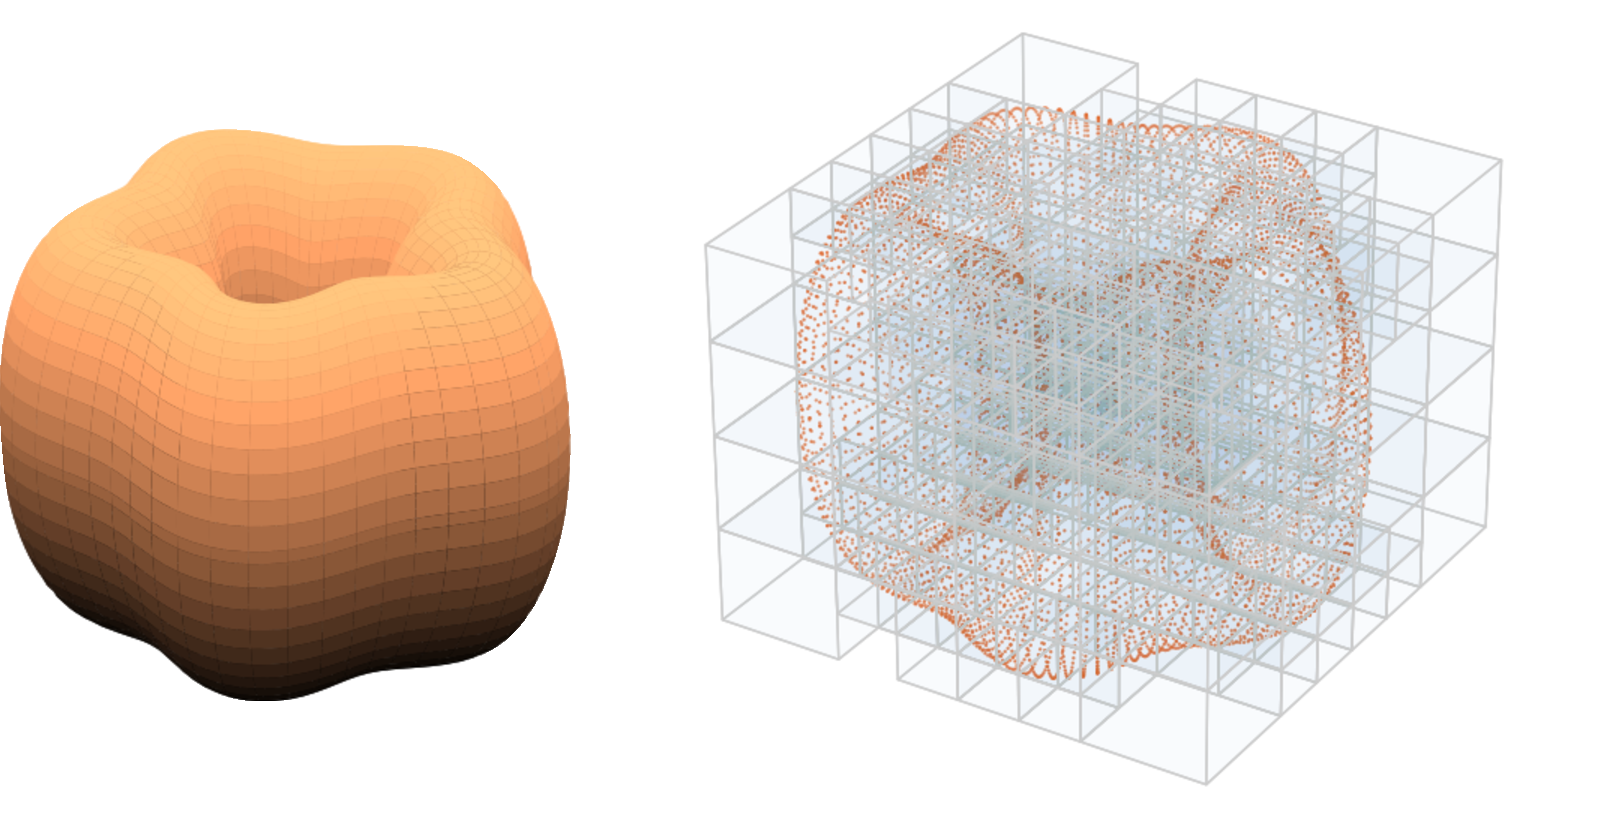
\includegraphics[width=0.7\textwidth]{ch_1/octree_example.pdf}
    \caption{An adaptive octree for random point data placed on the surface of a `wiggly torus' test geometry. The user defines the level of recursion via a threshold for the maximum number of particles in a given node.}
    \label{fig:octree_example:sec_1_2}
\end{figure}


The FMM then consists of three steps: tree construction, a preorder `bottom up' traveral, and a postorder `top down' traversal, made up of eight operators. P2M, M2L and L2P have been introduced, however we also require P2L, M2L, L2L, L2P, M2P and P2P, applied once to each applicable node. The operators define interactions between a given ‘target’ node, and potentially multiple ‘source’ nodes from the tree. They are read as ‘X to Y’, where ‘P’ stands for particle(s), ‘M’ for multipole expansion and ‘L’ for local expansion. The non-adaptive case is similar, except the $W$ and $X$ lists are now empty.

\begin{algorithm}
\caption{Fast Multipole Method}
\label{alg:fmm:sec_1_2}
\begin{algorithmic}

    \State $N$ is the total number of points
    \State $s$ is the maximum number of points in a leaf node.

    \State
    \State \textbf{Step 1: Tree construction}
    
    \For{each node $B$ in \textit{preorder} traversal of tree}
        \State subdivide $B$ if it contains more than $s$ points.
    \EndFor
    \For{each node $B$ in \textit{preorder} traversal of tree}
        \State construct \textit{interaction lists}, $U$, $V$, $X$, $W$
    \EndFor
    
    \State 
    \State \textbf{Step 2: Upward Pass}
    \For{each leaf node $B$ in \textit{postorder} traversal of the tree}
    \State \textbf{P2M}: compute multipole expansion for the particles they contain.
    \EndFor
    \For{each non leaf node $B$ in \textit{postorder} traversal of the tree}
    \State \textbf{M2M}: form a multipole expansion by translating and summing the expansion coefficients of the multipole expansions of its children.
    \EndFor

    \State
    \State \textbf{Step 3: Downward Pass}
    \For{each non-root node $B$ in \textit{preorder} traversal of the tree}
    \State \textbf{M2L}: translate multipole expansions of nodes in $B$'s $V$ list to a local expansion at $B$.
    \State \textbf{P2L}: translate the charges of particles in $B$'s $X$ to the local expansion at $B$.
    \State \textbf{L2L}: translate $B$'s local expansion to its children.
    \EndFor 

    \For{each leaf node $B$ in \textit{preorder} traversal of the tree}
    \State \textbf{P2P}: Directly compute the local interactions using the kernel between the particles in $B$ and its $U$ list.
    \State \textbf{L2P}: Translate local expansions for nodes in $B$'s $W$ list to the particles in $B$.
    \State \textbf{M2P}: Translate the multipole expansions for nodes in $B$'s $W$ list to the particles in $B$.
    \EndFor

\end{algorithmic}
\end{algorithm}

% In its original `analytical' form  \cite{greengard1987fast} an analytical series multipole expansion for a given node encoded point data within that node to a given expansion order, and the local expansion was the translation of this multipole expansion to another region of space in which it is analytic.

% As, the tree must be refined such that the leaf nodes contain only a small constant number of particles per leaf node, $s$, the maximum level of refinement is therefore approximately $n \approx \log(N)$, where $N$ is the number of particles in the tree. The multipole and local expansions are \textit{truncated} such that their expansion orders $p$, are chosen such that $p < N$,  the complexity of each translation operator (P2M, P2L, M2M, M2L, L2L, L2P, M2P) are bounded by complexities of the form $O(\kappa(p)N)$ where $\kappa(p)$ is a constant that depends on $p$, for all nodes in the tree. The direct calculations at the end are bounded by the maximum size of the $U$ lists, $|U|$, and $s$ as $O(s|U|N)$. The whole algorithm can therefore be seen to be bounded by $O(N)$. We defer to the literature for a more detailed analysis \cite{greengard1987fast}.


% The structure of the operators is the key difference between FMM implementations.

% - Note on how we've been deliberately vague on its implementation due to the variety of implementations. 
% - Need to have a note on how FMM actually works
% - Lead into the main differences between FMM implementations. 
% - Sketch out algebraic to analytic tagline, with a note on hierarchical methods.
% - Ambikasaran \& Darve summarise differences between different algebraic methods.
%     - H, H2, HSS, HBS, HODLR.


% - Comparison of analytical vs algebraic methods
% - Purely algebraic methods
%     - pre-compute and store entire hierarchical matrix.
%     - more storage, more data movement - both vertically and horizontally in memory hierarchy.
% - When the cost of data movement increases faster than arithmetic operations on future architectures, the methods that compute more to store/move less will become advantageous (computationally) - tradeoff results in KIFMM as choice - semi-analytical.

% - FMM vs other methods (FFT, Multigrid)
% - Uniform resolution use FFT, introduce FFT as first 'fast algorithm', however has unfavourable communication cost.
% - For non-uniform global problems also have multigrid methods as an alternative, also O(N) cost for elliptic/hyperbolic PDE problems. Gholami, Malhotra, Sundar, Biros (2016) - multigrid decent.

% - algebraic variants commonly argued to be superior as they operate directly on the matrix without the need to pass geometric information
%     - not convincing on their own.
%         - major libraries (PETSc) offer interfaces to insert a matrix free preconditioner as a function, and passing geometric info is something users are willing to do if it increases performance.
%     - Always just comes down to the flops vs bytes trade-off
%     - need a decent reference or description of where architecture technology is heading in order to justify our choice of FMM.

% - Note, analytical FMM have very high arithmetic intensity (flop/byte).
%     - not brute force methods doing wasteful calculations, only doing useful flops. Very different from achieving high arithmetic intensity on dense mat-mat mults or LU decompositions.
%     - Bonsai - an analytical treecode.

% - Fast translation operators crucial - take up a lot of time of the FMM, whatever its implementation.
%     - analytical options for fast translation operators.
%         - Rotation of spherical harmonics 92
%         - Block FFT 36
%         - Planewaves 50

%     - Accelerating M2L step
%         - level-skip M2L method 91
%         - 8,4,2 box method 93
%         - methods that use dual tree traversal alongside multipole acceptance criterion to construct optimal interaction lists 34

%     - Variable expansion order
%         - VFMM 85
%         - Guassian VFMM 20
%         - optimal parameter FMM 28
%     - intuition = boxes further away can afford to be of lower expansion order without loss of accuracy.

%     - Can store translations as matrices - typical optimisation
%         - matrix compression techniques - randomized techniques too.
%         - matrix techniques allow one to take advantage of BLAS
%             - maximises cache utilisation 39 (And US in PyExaFMM)
%         - Combination of techniques like Chebychev with SVD 38
%             - essentially systematic way of doing something like variable expansion order.
% - FMM is a method that has the analytical form to generate small (low-rank) off-diagonal matrices without needing to rely on a numerical approximation method.

% - making better use of translational invariance and rotational symmetry of the interaction list one can reduce the amount of storage further - 30, 32, 89

% - Lay out a sketch of the fast-algorithms for particle summation in terms of the flops/memory trade-off as in Yokota paper.

% - Discuss other hierarchical schemes (H, H2 etc) and explain why FMM is preferred for our application.

% - Explain why our version of FMM - semi-analytical - is preferred for programming.

% - Explain what we can focus on to really accelerate in the semi-analytical FMM to program for exascale, with reference to field translations chapter.

% - Discuss software construction for FMM, and what works and doesn't, what's currently available - and its shortcomings, and positives.

% - Discuss software challenges for high performance FMM, teeing up remaining sections of paper.

% - Close off with alternatives to FMM
% - Allows us to tackle problems that require non-uniform resolution, which isn't possible with the FFT
% - Multigrid methods - link to paper describing their performance.